\documentclass{book}
\usepackage[a4paper,top=2.5cm,bottom=2.5cm,left=2.5cm,right=2.5cm]{geometry}
\usepackage{makeidx}
\usepackage{natbib}
\usepackage{graphicx}
\usepackage{multicol}
\usepackage{float}
\usepackage{listings}
\usepackage{color}
\usepackage{ifthen}
\usepackage[table]{xcolor}
\usepackage{textcomp}
\usepackage{alltt}
\usepackage{ifpdf}
\ifpdf
\usepackage[pdftex,
            pagebackref=true,
            colorlinks=true,
            linkcolor=blue,
            unicode
           ]{hyperref}
\else
\usepackage[ps2pdf,
            pagebackref=true,
            colorlinks=true,
            linkcolor=blue,
            unicode
           ]{hyperref}
\usepackage{pspicture}
\fi
\usepackage[utf8]{inputenc}
\usepackage[french]{babel}

\usepackage{mathptmx}
\usepackage[scaled=.90]{helvet}
\usepackage{courier}
\usepackage{sectsty}
\usepackage{amssymb}
\usepackage[titles]{tocloft}
\usepackage{doxygen}
\lstset{language=C++,inputencoding=utf8,basicstyle=\footnotesize,breaklines=true,breakatwhitespace=true,tabsize=8,numbers=left }
\makeindex
\setcounter{tocdepth}{3}
\renewcommand{\footrulewidth}{0.4pt}
\renewcommand{\familydefault}{\sfdefault}
\hfuzz=15pt
\setlength{\emergencystretch}{15pt}
\hbadness=750
\tolerance=750
\begin{document}
\hypersetup{pageanchor=false,citecolor=blue}
\begin{titlepage}
\vspace*{7cm}
\begin{center}
{\Large Minecraft-\/\-Like \\[1ex]\large 1.\-5 }\\
\vspace*{1cm}
{\large Généré par Doxygen 1.8.1.2}\\
\vspace*{0.5cm}
{\small Jeudi Mars 21 2013 22:53:48}\\
\end{center}
\end{titlepage}
\clearemptydoublepage
\pagenumbering{roman}
\tableofcontents
\clearemptydoublepage
\pagenumbering{arabic}
\hypersetup{pageanchor=true,citecolor=blue}
\chapter{Index des espaces de nommage}
\section{Liste des espaces de nommage}
Liste de tous les espaces de nommage documentés avec une brève description\-:\begin{DoxyCompactList}
\item\contentsline{section}{\hyperlink{namespaceccli}{ccli} }{\pageref{namespaceccli}}{}
\end{DoxyCompactList}

\chapter{Index des classes}
\section{Hiérarchie des classes}
Cette liste d'héritage est classée approximativement par ordre alphabétique \-:\begin{DoxyCompactList}
\item \contentsline{section}{Camera}{\pageref{classCamera}}{}
\item \contentsline{section}{Client}{\pageref{classClient}}{}
\item \contentsline{section}{Controles}{\pageref{classControles}}{}
\item \contentsline{section}{Cube}{\pageref{classCube}}{}
\begin{DoxyCompactList}
\item \contentsline{section}{Cube\-Pelouse}{\pageref{classCubePelouse}}{}
\item \contentsline{section}{Cube\-Pierre}{\pageref{classCubePierre}}{}
\item \contentsline{section}{Cube\-Terre}{\pageref{classCubeTerre}}{}
\end{DoxyCompactList}
\item \contentsline{section}{Ecran}{\pageref{classEcran}}{}
\item \contentsline{section}{Face}{\pageref{classFace}}{}
\item \contentsline{section}{Joueur}{\pageref{classJoueur}}{}
\begin{DoxyCompactList}
\item \contentsline{section}{Joueur\-Ext}{\pageref{classJoueurExt}}{}
\end{DoxyCompactList}
\item \contentsline{section}{Membre}{\pageref{classMembre}}{}
\item \contentsline{section}{Networking\-Exception}{\pageref{classNetworkingException}}{}
\item \contentsline{section}{Personnage}{\pageref{classPersonnage}}{}
\item \contentsline{section}{Plateau}{\pageref{classPlateau}}{}
\item \contentsline{section}{Point}{\pageref{classPoint}}{}
\item \contentsline{section}{Serveur}{\pageref{classServeur}}{}
\end{DoxyCompactList}

\chapter{Index des classes}
\section{Liste des classes}
Liste des classes, structures, unions et interfaces avec une brève description \-:\begin{DoxyCompactList}
\item\contentsline{section}{\hyperlink{classCamera}{Camera} }{\pageref{classCamera}}{}
\item\contentsline{section}{\hyperlink{classClient}{Client} }{\pageref{classClient}}{}
\item\contentsline{section}{\hyperlink{classControles}{Controles} }{\pageref{classControles}}{}
\item\contentsline{section}{\hyperlink{classCube}{Cube} }{\pageref{classCube}}{}
\item\contentsline{section}{\hyperlink{classCubePelouse}{Cube\-Pelouse} }{\pageref{classCubePelouse}}{}
\item\contentsline{section}{\hyperlink{classCubePierre}{Cube\-Pierre} }{\pageref{classCubePierre}}{}
\item\contentsline{section}{\hyperlink{classCubeTerre}{Cube\-Terre} }{\pageref{classCubeTerre}}{}
\item\contentsline{section}{\hyperlink{classEcran}{Ecran} }{\pageref{classEcran}}{}
\item\contentsline{section}{\hyperlink{classFace}{Face} }{\pageref{classFace}}{}
\item\contentsline{section}{\hyperlink{classJoueur}{Joueur} }{\pageref{classJoueur}}{}
\item\contentsline{section}{\hyperlink{classJoueurExt}{Joueur\-Ext} }{\pageref{classJoueurExt}}{}
\item\contentsline{section}{\hyperlink{classMembre}{Membre} }{\pageref{classMembre}}{}
\item\contentsline{section}{\hyperlink{classNetworkingException}{Networking\-Exception} }{\pageref{classNetworkingException}}{}
\item\contentsline{section}{\hyperlink{classPersonnage}{Personnage} }{\pageref{classPersonnage}}{}
\item\contentsline{section}{\hyperlink{classPlateau}{Plateau} }{\pageref{classPlateau}}{}
\item\contentsline{section}{\hyperlink{classPoint}{Point} }{\pageref{classPoint}}{}
\item\contentsline{section}{\hyperlink{classServeur}{Serveur} }{\pageref{classServeur}}{}
\end{DoxyCompactList}

\chapter{Documentation des espaces de nommage}
\hypertarget{namespaceccli}{\section{Référence de l'espace de nommage ccli}
\label{namespaceccli}\index{ccli@{ccli}}
}
\subsection*{Variables}
\begin{DoxyCompactItemize}
\item 
\hypertarget{namespaceccli_abd9b5c419c288a34236b2e31a58bac3e}{std\-::mutex {\bfseries ms}}\label{namespaceccli_abd9b5c419c288a34236b2e31a58bac3e}

\end{DoxyCompactItemize}


\subsection{Description détaillée}
Namespace client 
\chapter{Documentation des classes}
\hypertarget{classCamera}{\section{Référence de la classe Camera}
\label{classCamera}\index{Camera@{Camera}}
}
\subsection*{Fonctions membres publiques}
\begin{DoxyCompactItemize}
\item 
\hypertarget{classCamera_acf7c600a4689b20bfffbefa28fc04a23}{{\bfseries Camera} (int, int, int)}\label{classCamera_acf7c600a4689b20bfffbefa28fc04a23}

\item 
\hypertarget{classCamera_abc7336dba615440cc6565c09f77bd238}{void {\bfseries avancer} (float, float)}\label{classCamera_abc7336dba615440cc6565c09f77bd238}

\item 
\hypertarget{classCamera_abcdf75028bddba769241f89848d53e3f}{void {\bfseries reculer} (float, float)}\label{classCamera_abcdf75028bddba769241f89848d53e3f}

\item 
\hypertarget{classCamera_affc06966e025a837540d637177d7378c}{void {\bfseries maj} (float, float)}\label{classCamera_affc06966e025a837540d637177d7378c}

\item 
\hypertarget{classCamera_a9929a922055dda4e2e68931ca785792d}{float {\bfseries get\-Posx} ()}\label{classCamera_a9929a922055dda4e2e68931ca785792d}

\item 
\hypertarget{classCamera_a20ea0f1711dd5167b1490eca6368fdb3}{float {\bfseries get\-Posy} ()}\label{classCamera_a20ea0f1711dd5167b1490eca6368fdb3}

\item 
\hypertarget{classCamera_ae49efb8343381e6e842a36471ce47ced}{float {\bfseries get\-Posz} ()}\label{classCamera_ae49efb8343381e6e842a36471ce47ced}

\end{DoxyCompactItemize}


La documentation de cette classe a été générée à partir des fichiers suivants \-:\begin{DoxyCompactItemize}
\item 
/home/xyrodileas/\-Bureau/\-Projet\-\_\-\-Graphique/trunk/code\-\_\-source/src/graphique/Camera.\-h\item 
/home/xyrodileas/\-Bureau/\-Projet\-\_\-\-Graphique/trunk/code\-\_\-source/src/graphique/Camera.\-cpp\end{DoxyCompactItemize}

\hypertarget{classClient}{\section{Référence de la classe Client}
\label{classClient}\index{Client@{Client}}
}


{\ttfamily \#include $<$reseau.\-hpp$>$}

\subsection*{Fonctions membres publiques}
\begin{DoxyCompactItemize}
\item 
\hyperlink{classClient_af7faf381e7062b0135ab53c35dbb5542}{Client} (std\-::string)
\item 
void \hyperlink{classClient_ababa7bdcba8521f9a696711446d47e04}{envoyer} (std\-::string)
\item 
std\-::string \hyperlink{classClient_a7ec691731f5b7d5accc7dcd9d585ad4d}{recevoir} ()
\item 
\hypertarget{classClient_a203aac6c2bb9ae7d140c62d7ae836718}{void {\bfseries quitter} ()}\label{classClient_a203aac6c2bb9ae7d140c62d7ae836718}

\item 
\hyperlink{classClient_a840e519ca781888cbd54181572ebe3a7}{$\sim$\-Client} ()
\end{DoxyCompactItemize}
\subsection*{Amis}
\begin{DoxyCompactItemize}
\item 
void $\ast$ \hyperlink{classClient_a748a40bc18d4ed6e2f98f1e9908f8711}{envoi} (void $\ast$)
\item 
void $\ast$ \hyperlink{classClient_aeaf2388f2f63df46fb9a90f59c34db91}{recu} (void $\ast$)
\end{DoxyCompactItemize}


\subsection{Description détaillée}
La classe cliente est beaucoup plus simple puisqu'elle se connecte, envoie et recoit des informations de deux type possible et c'est tout ! 

\subsection{Documentation des constructeurs et destructeur}
\hypertarget{classClient_af7faf381e7062b0135ab53c35dbb5542}{\index{Client@{Client}!Client@{Client}}
\index{Client@{Client}!Client@{Client}}
\subsubsection[{Client}]{\setlength{\rightskip}{0pt plus 5cm}Client\-::\-Client (
\begin{DoxyParamCaption}
\item[{std\-::string}]{nom}
\end{DoxyParamCaption}
)}}\label{classClient_af7faf381e7062b0135ab53c35dbb5542}
Constructeur, Se connecte au serveur et attend des messages dans un thread \hypertarget{classClient_a840e519ca781888cbd54181572ebe3a7}{\index{Client@{Client}!$\sim$\-Client@{$\sim$\-Client}}
\index{$\sim$\-Client@{$\sim$\-Client}!Client@{Client}}
\subsubsection[{$\sim$\-Client}]{\setlength{\rightskip}{0pt plus 5cm}Client\-::$\sim$\-Client (
\begin{DoxyParamCaption}
{}
\end{DoxyParamCaption}
)}}\label{classClient_a840e519ca781888cbd54181572ebe3a7}
Destructeur classique 

\subsection{Documentation des fonctions membres}
\hypertarget{classClient_ababa7bdcba8521f9a696711446d47e04}{\index{Client@{Client}!envoyer@{envoyer}}
\index{envoyer@{envoyer}!Client@{Client}}
\subsubsection[{envoyer}]{\setlength{\rightskip}{0pt plus 5cm}void Client\-::envoyer (
\begin{DoxyParamCaption}
\item[{std\-::string}]{mess}
\end{DoxyParamCaption}
)}}\label{classClient_ababa7bdcba8521f9a696711446d47e04}
ne pas croire que \hyperlink{classClient_ababa7bdcba8521f9a696711446d47e04}{envoyer()} envoi sur le reseau, cela se fait avec des fonctions prive envoi met votre message sur une liste d'attente pour etre envoye \hypertarget{classClient_a7ec691731f5b7d5accc7dcd9d585ad4d}{\index{Client@{Client}!recevoir@{recevoir}}
\index{recevoir@{recevoir}!Client@{Client}}
\subsubsection[{recevoir}]{\setlength{\rightskip}{0pt plus 5cm}std\-::string Client\-::recevoir (
\begin{DoxyParamCaption}
{}
\end{DoxyParamCaption}
)}}\label{classClient_a7ec691731f5b7d5accc7dcd9d585ad4d}
La reception est la recuperation des dernieres donne recu et mise dans un file par autres clients 

\subsection{Documentation des fonctions amies et associées}
\hypertarget{classClient_a748a40bc18d4ed6e2f98f1e9908f8711}{\index{Client@{Client}!envoi@{envoi}}
\index{envoi@{envoi}!Client@{Client}}
\subsubsection[{envoi}]{\setlength{\rightskip}{0pt plus 5cm}void$\ast$ envoi (
\begin{DoxyParamCaption}
\item[{void $\ast$}]{arg}
\end{DoxyParamCaption}
)\hspace{0.3cm}{\ttfamily [friend]}}}\label{classClient_a748a40bc18d4ed6e2f98f1e9908f8711}
Recupere les messages et les envoie au serveur \hypertarget{classClient_aeaf2388f2f63df46fb9a90f59c34db91}{\index{Client@{Client}!recu@{recu}}
\index{recu@{recu}!Client@{Client}}
\subsubsection[{recu}]{\setlength{\rightskip}{0pt plus 5cm}void$\ast$ recu (
\begin{DoxyParamCaption}
\item[{void $\ast$}]{arg}
\end{DoxyParamCaption}
)\hspace{0.3cm}{\ttfamily [friend]}}}\label{classClient_aeaf2388f2f63df46fb9a90f59c34db91}
Recupere les messages du serveur et les rend diponible par le client 

La documentation de cette classe a été générée à partir des fichiers suivants \-:\begin{DoxyCompactItemize}
\item 
/home/xyrodileas/\-Bureau/\-Projet\-\_\-\-Graphique/trunk/code\-\_\-source/src/reseau/reseau.\-hpp\item 
/home/xyrodileas/\-Bureau/\-Projet\-\_\-\-Graphique/trunk/code\-\_\-source/src/reseau/client.\-cpp\end{DoxyCompactItemize}

\hypertarget{classControles}{\section{Référence de la classe Controles}
\label{classControles}\index{Controles@{Controles}}
}
\subsection*{Fonctions membres publiques}
\begin{DoxyCompactItemize}
\item 
\hypertarget{classControles_a85c346918567b55c260ece35d75f3ce8}{{\bfseries Controles} (int)}\label{classControles_a85c346918567b55c260ece35d75f3ce8}

\item 
\hypertarget{classControles_a1cf794967c60914ef9ad22f61bad2525}{void \hyperlink{classControles_a1cf794967c60914ef9ad22f61bad2525}{Check} (const sf\-::\-Input \&Input)}\label{classControles_a1cf794967c60914ef9ad22f61bad2525}

\begin{DoxyCompactList}\small\item\em Vérifie l'état des touches de contrôles. \end{DoxyCompactList}\item 
\hypertarget{classControles_a570494eca52fa3194d52d04f79d1ca17}{void \hyperlink{classControles_a570494eca52fa3194d52d04f79d1ca17}{Action} (\hyperlink{classJoueur}{Joueur} \&, \hyperlink{classPlateau}{Plateau} \&, float)}\label{classControles_a570494eca52fa3194d52d04f79d1ca17}

\begin{DoxyCompactList}\small\item\em Applique les actions à faire en fonction des contrôles actionné \end{DoxyCompactList}\item 
\hypertarget{classControles_a8e3d0dc550191ba752203885a6f848fe}{float {\bfseries get\-Anglex} ()}\label{classControles_a8e3d0dc550191ba752203885a6f848fe}

\item 
\hypertarget{classControles_ab22968993b4f4b136c58c7276395f773}{float {\bfseries get\-Angley} ()}\label{classControles_ab22968993b4f4b136c58c7276395f773}

\item 
\hypertarget{classControles_adfcb548e36751cf333c8f465a688e7d9}{void \hyperlink{classControles_adfcb548e36751cf333c8f465a688e7d9}{Sauter} (\hyperlink{classJoueur}{Joueur} \&, \hyperlink{classPlateau}{Plateau} \&)}\label{classControles_adfcb548e36751cf333c8f465a688e7d9}

\begin{DoxyCompactList}\small\item\em Permet de faire sauter le joueur. \end{DoxyCompactList}\end{DoxyCompactItemize}
\subsection*{Attributs publics}
\begin{DoxyCompactItemize}
\item 
\hypertarget{classControles_aafce4f25afb7cb49684dfde3f4c1f5db}{float {\bfseries anglex}}\label{classControles_aafce4f25afb7cb49684dfde3f4c1f5db}

\item 
\hypertarget{classControles_a304b1a6acbc7a488a1576e279696e967}{float {\bfseries angley}}\label{classControles_a304b1a6acbc7a488a1576e279696e967}

\end{DoxyCompactItemize}


La documentation de cette classe a été générée à partir des fichiers suivants \-:\begin{DoxyCompactItemize}
\item 
/home/xyrodileas/\-Bureau/\-Projet\-\_\-\-Graphique/trunk/code\-\_\-source/src/\-Joueur/Controles.\-h\item 
/home/xyrodileas/\-Bureau/\-Projet\-\_\-\-Graphique/trunk/code\-\_\-source/src/\-Joueur/Controles.\-cpp\end{DoxyCompactItemize}

\hypertarget{classCube}{\section{Référence de la classe Cube}
\label{classCube}\index{Cube@{Cube}}
}
Graphe d'héritage de Cube\-:\begin{figure}[H]
\begin{center}
\leavevmode
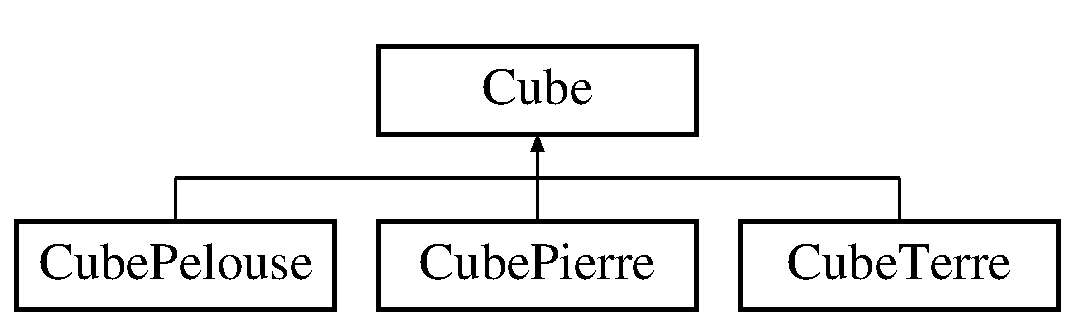
\includegraphics[height=2.000000cm]{classCube}
\end{center}
\end{figure}
\subsection*{Fonctions membres publiques}
\begin{DoxyCompactItemize}
\item 
\hypertarget{classCube_aff3bf4c9ea1a38e10c646aa39d363eca}{{\bfseries Cube} (int, int, int, float, int, int, int, bool, bool, bool, bool, bool, bool)}\label{classCube_aff3bf4c9ea1a38e10c646aa39d363eca}

\item 
\hypertarget{classCube_aa04ef7154adc3feefa0ebb09f3628f37}{void \hyperlink{classCube_aa04ef7154adc3feefa0ebb09f3628f37}{construire\-\_\-cube} ()}\label{classCube_aa04ef7154adc3feefa0ebb09f3628f37}

\begin{DoxyCompactList}\small\item\em Permet de construire un cube en affichant uniquement les faces visibles. \end{DoxyCompactList}\item 
\hypertarget{classCube_ac39c5f7f1fdc8ee24546782c67da73ae}{void {\bfseries afficher\-\_\-avant} (bool affiche\-Avant)}\label{classCube_ac39c5f7f1fdc8ee24546782c67da73ae}

\item 
\hypertarget{classCube_ac7a896d3041c09dc2e0554e9e26b5ca1}{void {\bfseries afficher\-\_\-arriere} (bool affiche\-Arriere)}\label{classCube_ac7a896d3041c09dc2e0554e9e26b5ca1}

\item 
\hypertarget{classCube_a2628233ae02c22edc27063894a861389}{void {\bfseries afficher\-\_\-dessous} (bool affiche\-Dessous)}\label{classCube_a2628233ae02c22edc27063894a861389}

\item 
\hypertarget{classCube_aa1bcd3527d9fe2006ba467c3a5d2040a}{void {\bfseries afficher\-\_\-dessus} (bool affiche\-Dessus)}\label{classCube_aa1bcd3527d9fe2006ba467c3a5d2040a}

\item 
\hypertarget{classCube_a468f17645009f9dd36906bfde0ee4c8b}{void {\bfseries afficher\-\_\-gauche} (bool affiche\-Gauche)}\label{classCube_a468f17645009f9dd36906bfde0ee4c8b}

\item 
\hypertarget{classCube_ad4973e18267f1d452fd49829bb370b3d}{void {\bfseries afficher\-\_\-droite} (bool affiche\-Droite)}\label{classCube_ad4973e18267f1d452fd49829bb370b3d}

\item 
\hypertarget{classCube_a533025489332814204d81a90672741df}{int {\bfseries get\-X} ()}\label{classCube_a533025489332814204d81a90672741df}

\item 
\hypertarget{classCube_ab4e951c24701feed0b63ce63cb7e8c97}{int {\bfseries get\-Y} ()}\label{classCube_ab4e951c24701feed0b63ce63cb7e8c97}

\item 
\hypertarget{classCube_a803a27c6e5dc68770127f44295f9416c}{int {\bfseries get\-Z} ()}\label{classCube_a803a27c6e5dc68770127f44295f9416c}

\item 
\hypertarget{classCube_a70621eb12f52a957af2788fbdb6ec76e}{int {\bfseries get\-Taille} ()}\label{classCube_a70621eb12f52a957af2788fbdb6ec76e}

\item 
\hypertarget{classCube_a4f9079c9c5d882924d9c626dc655a60f}{int {\bfseries get\-Rouge} ()}\label{classCube_a4f9079c9c5d882924d9c626dc655a60f}

\item 
\hypertarget{classCube_a32a5e44317458720135c32feb2801d43}{int {\bfseries get\-Vert} ()}\label{classCube_a32a5e44317458720135c32feb2801d43}

\item 
\hypertarget{classCube_a37388ae818ea4a24abce5910d1d7fd5d}{int {\bfseries get\-Bleu} ()}\label{classCube_a37388ae818ea4a24abce5910d1d7fd5d}

\end{DoxyCompactItemize}
\subsection*{Fonctions membres protégées}
\begin{DoxyCompactItemize}
\item 
\hypertarget{classCube_a5e4ade27eddade88c60cafe3889be95b}{void \hyperlink{classCube_a5e4ade27eddade88c60cafe3889be95b}{initialiser\-\_\-cube} ()}\label{classCube_a5e4ade27eddade88c60cafe3889be95b}

\begin{DoxyCompactList}\small\item\em Initialise les faces d'un cube. \end{DoxyCompactList}\end{DoxyCompactItemize}
\subsection*{Attributs protégés}
\begin{DoxyCompactItemize}
\item 
\hypertarget{classCube_aa4f56a40ada8a030ac48d775d2ac6ad1}{int {\bfseries x}}\label{classCube_aa4f56a40ada8a030ac48d775d2ac6ad1}

\item 
\hypertarget{classCube_a0d4c859ce871ed5eb4d02a83823a77f9}{int {\bfseries y}}\label{classCube_a0d4c859ce871ed5eb4d02a83823a77f9}

\item 
\hypertarget{classCube_a181171a5a8434e8eef79b3308ae08e03}{int {\bfseries z}}\label{classCube_a181171a5a8434e8eef79b3308ae08e03}

\item 
\hypertarget{classCube_a70f3132d99958062f45499c5453fd959}{float {\bfseries taille}}\label{classCube_a70f3132d99958062f45499c5453fd959}

\item 
\hypertarget{classCube_a174baf27071a6f70d5f12ab798ed186c}{int {\bfseries rouge}}\label{classCube_a174baf27071a6f70d5f12ab798ed186c}

\item 
\hypertarget{classCube_aa99801491d1f8e7b220465e4e9d54c0f}{int {\bfseries vert}}\label{classCube_aa99801491d1f8e7b220465e4e9d54c0f}

\item 
\hypertarget{classCube_ab7d03764d207dc8c29e4a4b99109063c}{int {\bfseries bleu}}\label{classCube_ab7d03764d207dc8c29e4a4b99109063c}

\item 
\hypertarget{classCube_adceb9f70f2cc8322ecf49342f514cc75}{\hyperlink{classFace}{Face} $\ast$ {\bfseries avant}}\label{classCube_adceb9f70f2cc8322ecf49342f514cc75}

\item 
\hypertarget{classCube_aab5a1291adfb387abd49893dd9a7097f}{\hyperlink{classFace}{Face} $\ast$ {\bfseries arriere}}\label{classCube_aab5a1291adfb387abd49893dd9a7097f}

\item 
\hypertarget{classCube_a112099089b84e89f60d77740fe7c5120}{\hyperlink{classFace}{Face} $\ast$ {\bfseries dessous}}\label{classCube_a112099089b84e89f60d77740fe7c5120}

\item 
\hypertarget{classCube_a39e112f9a2d9c9ead7d9493624733784}{\hyperlink{classFace}{Face} $\ast$ {\bfseries dessus}}\label{classCube_a39e112f9a2d9c9ead7d9493624733784}

\item 
\hypertarget{classCube_a20f3cdf33801cd347159274dfe15309e}{\hyperlink{classFace}{Face} $\ast$ {\bfseries gauche}}\label{classCube_a20f3cdf33801cd347159274dfe15309e}

\item 
\hypertarget{classCube_a9c1fcb84ad9d36212e381a2ac106726d}{\hyperlink{classFace}{Face} $\ast$ {\bfseries droite}}\label{classCube_a9c1fcb84ad9d36212e381a2ac106726d}

\item 
\hypertarget{classCube_a9da9d67b27b32955b66d2c6c92eae794}{bool {\bfseries affiche\-Avant}}\label{classCube_a9da9d67b27b32955b66d2c6c92eae794}

\item 
\hypertarget{classCube_a30e384bb71aa9b3ebc25c03bef785815}{bool {\bfseries affiche\-Arriere}}\label{classCube_a30e384bb71aa9b3ebc25c03bef785815}

\item 
\hypertarget{classCube_a39fa6217cd00765fe3f14c46fee39f28}{bool {\bfseries affiche\-Dessous}}\label{classCube_a39fa6217cd00765fe3f14c46fee39f28}

\item 
\hypertarget{classCube_aef7d564ad9783a84b17226e99c88f06c}{bool {\bfseries affiche\-Dessus}}\label{classCube_aef7d564ad9783a84b17226e99c88f06c}

\item 
\hypertarget{classCube_ad7012c8e174b39e23de36f78e73e0f95}{bool {\bfseries affiche\-Gauche}}\label{classCube_ad7012c8e174b39e23de36f78e73e0f95}

\item 
\hypertarget{classCube_aa98904d1d3f776620b50a3608d6da818}{bool {\bfseries affiche\-Droite}}\label{classCube_aa98904d1d3f776620b50a3608d6da818}

\end{DoxyCompactItemize}


La documentation de cette classe a été générée à partir des fichiers suivants \-:\begin{DoxyCompactItemize}
\item 
/home/xyrodileas/\-Bureau/\-Projet\-\_\-\-Graphique/trunk/code\-\_\-source/src/cube/Cube.\-h\item 
/home/xyrodileas/\-Bureau/\-Projet\-\_\-\-Graphique/trunk/code\-\_\-source/src/cube/Cube.\-cpp\end{DoxyCompactItemize}

\hypertarget{classCubePelouse}{\section{Référence de la classe Cube\-Pelouse}
\label{classCubePelouse}\index{Cube\-Pelouse@{Cube\-Pelouse}}
}
Graphe d'héritage de Cube\-Pelouse\-:\begin{figure}[H]
\begin{center}
\leavevmode
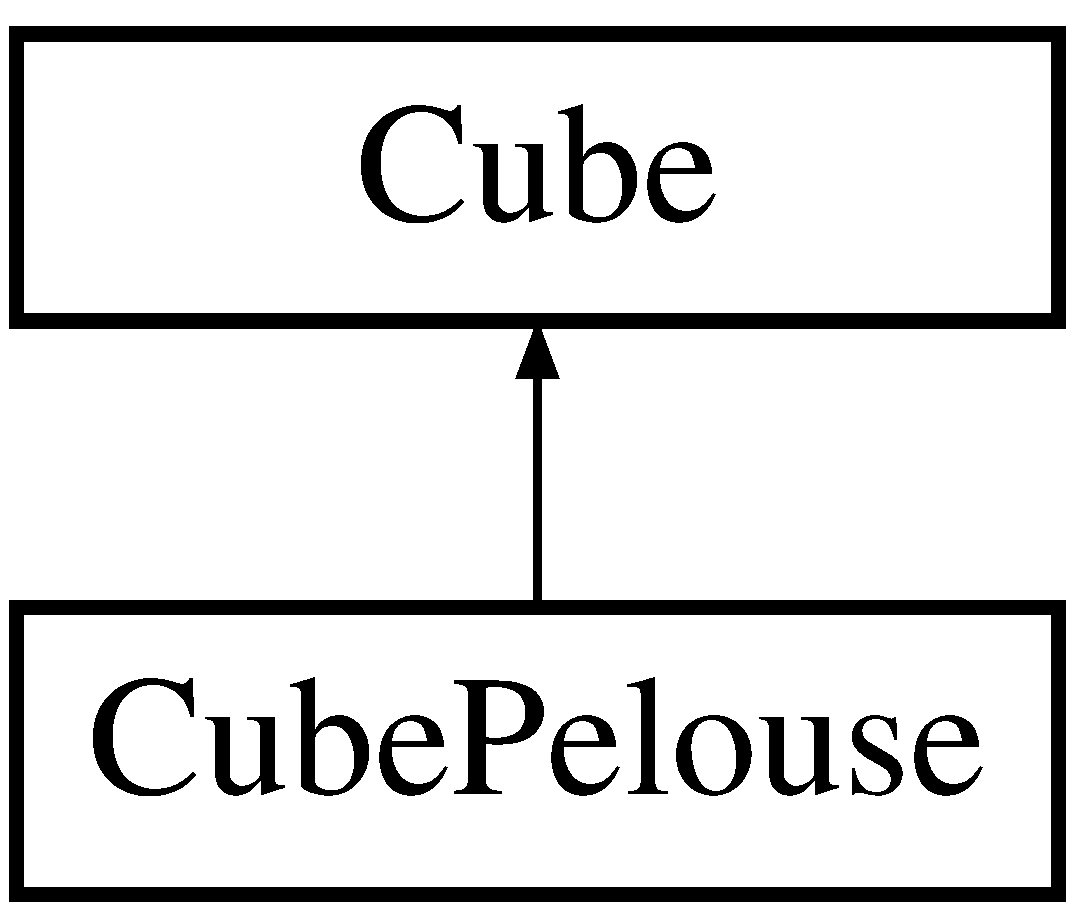
\includegraphics[height=2.000000cm]{classCubePelouse}
\end{center}
\end{figure}
\subsection*{Fonctions membres publiques}
\begin{DoxyCompactItemize}
\item 
\hypertarget{classCubePelouse_a501b5442ea45c7f53d7e34d5d80b3387}{{\bfseries Cube\-Pelouse} (int, int, int, float, bool, bool, bool, bool, bool, bool)}\label{classCubePelouse_a501b5442ea45c7f53d7e34d5d80b3387}

\end{DoxyCompactItemize}
\subsection*{Additional Inherited Members}


La documentation de cette classe a été générée à partir des fichiers suivants \-:\begin{DoxyCompactItemize}
\item 
/home/xyrodileas/\-Bureau/\-Projet\-\_\-\-Graphique/trunk/code\-\_\-source/src/cube/type\-\_\-cube/Cube\-Pelouse.\-h\item 
/home/xyrodileas/\-Bureau/\-Projet\-\_\-\-Graphique/trunk/code\-\_\-source/src/cube/type\-\_\-cube/Cube\-Pelouse.\-cpp\end{DoxyCompactItemize}

\hypertarget{classCubePierre}{\section{Référence de la classe Cube\-Pierre}
\label{classCubePierre}\index{Cube\-Pierre@{Cube\-Pierre}}
}
Graphe d'héritage de Cube\-Pierre\-:\begin{figure}[H]
\begin{center}
\leavevmode
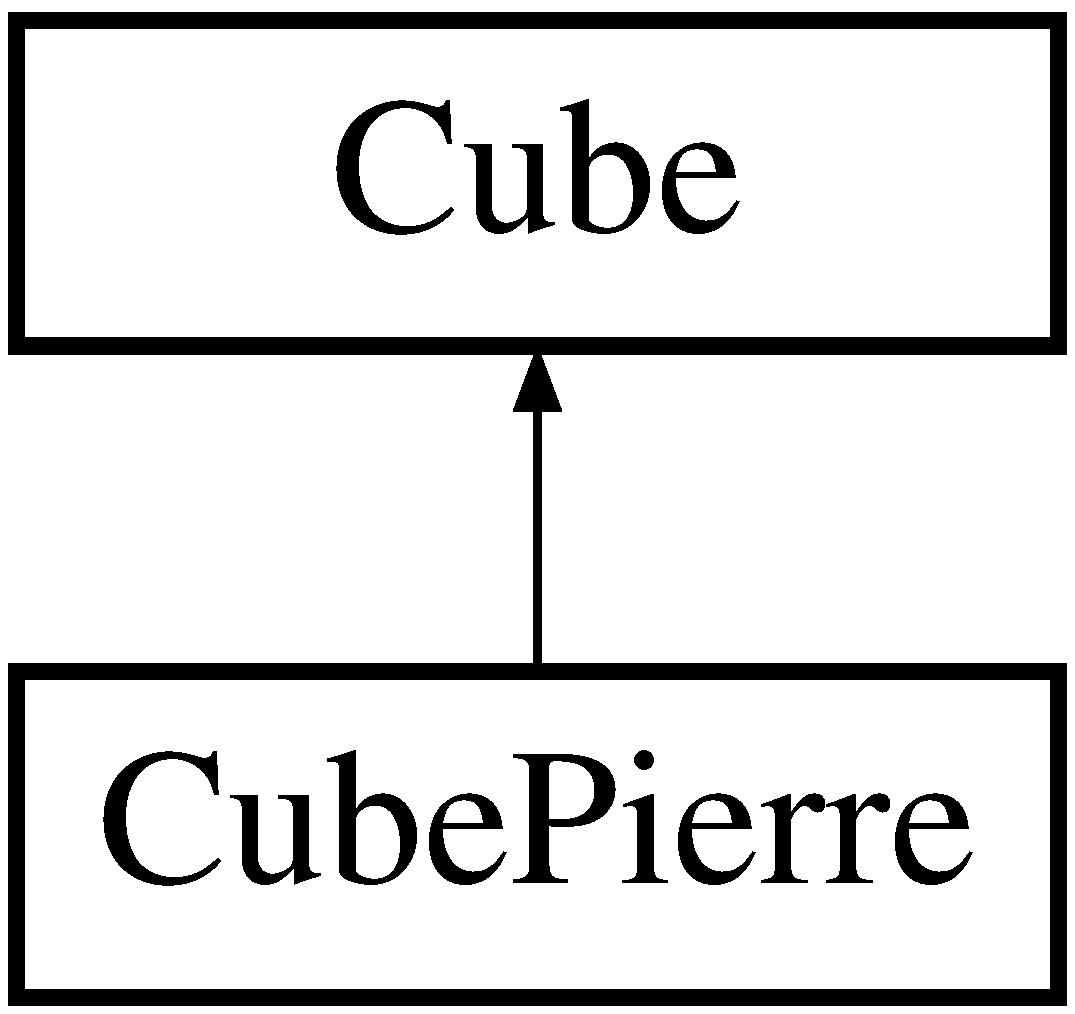
\includegraphics[height=2.000000cm]{classCubePierre}
\end{center}
\end{figure}
\subsection*{Fonctions membres publiques}
\begin{DoxyCompactItemize}
\item 
\hypertarget{classCubePierre_a229ef3b4612798a0deba792041e528ba}{{\bfseries Cube\-Pierre} (int, int, int, float, bool, bool, bool, bool, bool, bool)}\label{classCubePierre_a229ef3b4612798a0deba792041e528ba}

\end{DoxyCompactItemize}
\subsection*{Additional Inherited Members}


La documentation de cette classe a été générée à partir des fichiers suivants \-:\begin{DoxyCompactItemize}
\item 
/home/xyrodileas/\-Bureau/\-Projet\-\_\-\-Graphique/trunk/code\-\_\-source/src/cube/type\-\_\-cube/Cube\-Pierre.\-h\item 
/home/xyrodileas/\-Bureau/\-Projet\-\_\-\-Graphique/trunk/code\-\_\-source/src/cube/type\-\_\-cube/Cube\-Pierre.\-cpp\end{DoxyCompactItemize}

\hypertarget{classCubeTerre}{\section{Référence de la classe Cube\-Terre}
\label{classCubeTerre}\index{Cube\-Terre@{Cube\-Terre}}
}
Graphe d'héritage de Cube\-Terre\-:\begin{figure}[H]
\begin{center}
\leavevmode
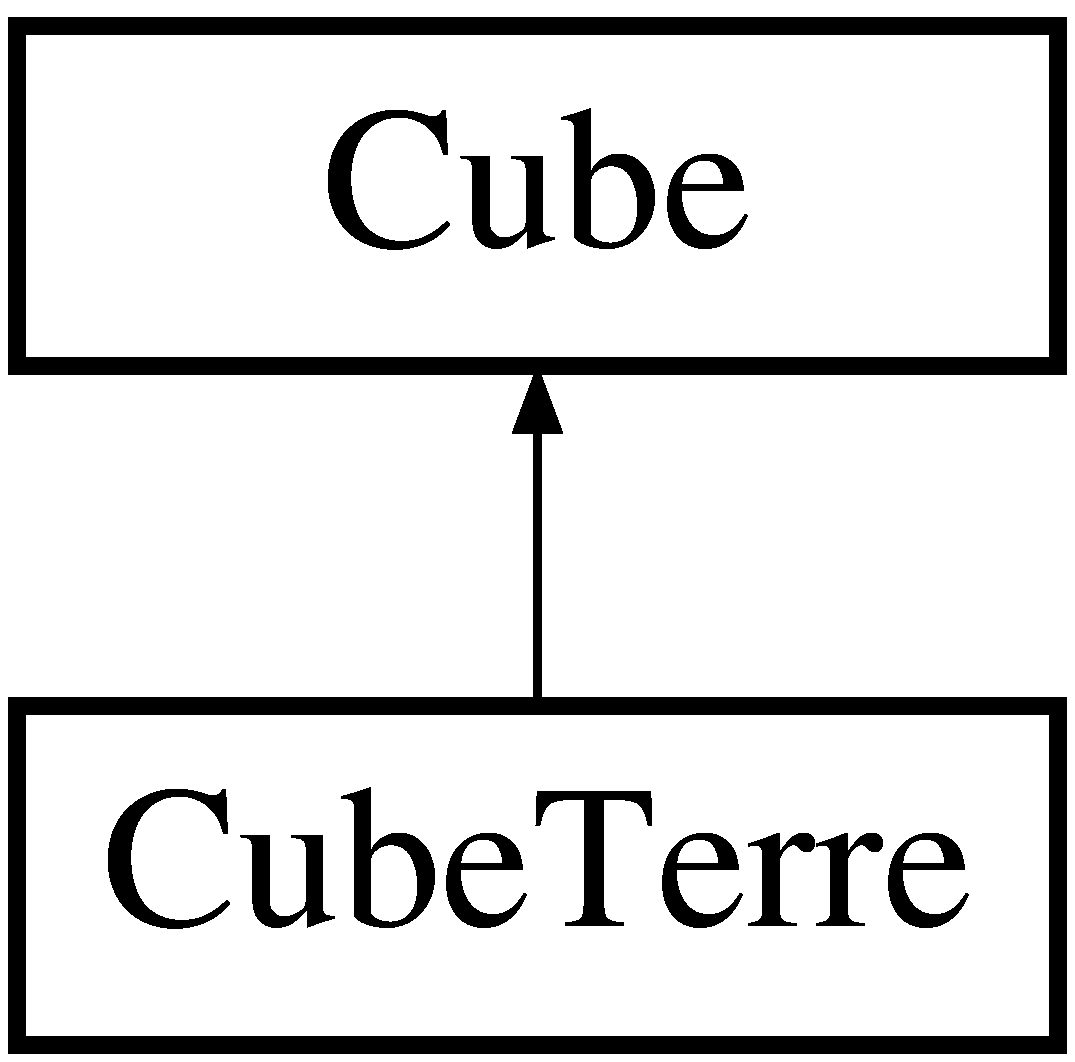
\includegraphics[height=2.000000cm]{classCubeTerre}
\end{center}
\end{figure}
\subsection*{Fonctions membres publiques}
\begin{DoxyCompactItemize}
\item 
\hypertarget{classCubeTerre_a475c94a1b7537cd9c7ad8328897ab3df}{{\bfseries Cube\-Terre} (int, int, int, float, bool, bool, bool, bool, bool, bool)}\label{classCubeTerre_a475c94a1b7537cd9c7ad8328897ab3df}

\end{DoxyCompactItemize}
\subsection*{Additional Inherited Members}


La documentation de cette classe a été générée à partir des fichiers suivants \-:\begin{DoxyCompactItemize}
\item 
/home/xyrodileas/\-Bureau/\-Projet\-\_\-\-Graphique/trunk/code\-\_\-source/src/cube/type\-\_\-cube/Cube\-Terre.\-h\item 
/home/xyrodileas/\-Bureau/\-Projet\-\_\-\-Graphique/trunk/code\-\_\-source/src/cube/type\-\_\-cube/Cube\-Terre.\-cpp\end{DoxyCompactItemize}

\hypertarget{classEcran}{\section{Référence de la classe Ecran}
\label{classEcran}\index{Ecran@{Ecran}}
}
\subsection*{Fonctions membres publiques}
\begin{DoxyCompactItemize}
\item 
\hypertarget{classEcran_aa5e60921af4bde1feab393bdcb58a8e2}{virtual {\bfseries $\sim$\-Ecran} (int, int, char $\ast$)}\label{classEcran_aa5e60921af4bde1feab393bdcb58a8e2}

\item 
\hypertarget{classEcran_a92a1ca31ca57e792a9e1b7d8cf0900ba}{void {\bfseries dessiner} ()}\label{classEcran_a92a1ca31ca57e792a9e1b7d8cf0900ba}

\end{DoxyCompactItemize}


La documentation de cette classe a été générée à partir des fichiers suivants \-:\begin{DoxyCompactItemize}
\item 
/home/xyrodileas/\-Bureau/\-Projet\-\_\-\-Graphique/trunk/code\-\_\-source/src/graphique/Ecran.\-h\item 
/home/xyrodileas/\-Bureau/\-Projet\-\_\-\-Graphique/trunk/code\-\_\-source/src/graphique/Ecran.\-cpp\end{DoxyCompactItemize}

\hypertarget{classFace}{\section{Référence de la classe Face}
\label{classFace}\index{Face@{Face}}
}
\subsection*{Fonctions membres publiques}
\begin{DoxyCompactItemize}
\item 
\hypertarget{classFace_a0d5b793f0b5f3b3f5b2bdb9350ab0f5e}{{\bfseries Face} (\hyperlink{classPoint}{Point}, \hyperlink{classPoint}{Point}, \hyperlink{classPoint}{Point}, \hyperlink{classPoint}{Point}, int, int, int)}\label{classFace_a0d5b793f0b5f3b3f5b2bdb9350ab0f5e}

\item 
\hypertarget{classFace_a3388255c476883e6c35af3f2a8e12a27}{void \hyperlink{classFace_a3388255c476883e6c35af3f2a8e12a27}{construire\-\_\-face} ()}\label{classFace_a3388255c476883e6c35af3f2a8e12a27}

\begin{DoxyCompactList}\small\item\em \textbackslash{} Permet de construire une face \end{DoxyCompactList}\end{DoxyCompactItemize}
\subsection*{Attributs protégés}
\begin{DoxyCompactItemize}
\item 
\hypertarget{classFace_a6347208958acabe7c1e07660a8016991}{\hyperlink{classPoint}{Point} {\bfseries point}}\label{classFace_a6347208958acabe7c1e07660a8016991}

\item 
\hypertarget{classFace_a53180d3d69a7e064b5a98e84314f73c2}{\hyperlink{classPoint}{Point} {\bfseries point2}}\label{classFace_a53180d3d69a7e064b5a98e84314f73c2}

\item 
\hypertarget{classFace_a7928a2f75a5e4cb7909e3decf0a1953f}{\hyperlink{classPoint}{Point} {\bfseries point3}}\label{classFace_a7928a2f75a5e4cb7909e3decf0a1953f}

\item 
\hypertarget{classFace_ad3d69dea20bb9f184f83d80cb0f1fa48}{\hyperlink{classPoint}{Point} {\bfseries point4}}\label{classFace_ad3d69dea20bb9f184f83d80cb0f1fa48}

\item 
\hypertarget{classFace_aaa3a01311d47934fd138dfa96577ec5f}{float {\bfseries taille}}\label{classFace_aaa3a01311d47934fd138dfa96577ec5f}

\item 
\hypertarget{classFace_a238c37178677fda653c8c920fb1d89f8}{int {\bfseries rouge}}\label{classFace_a238c37178677fda653c8c920fb1d89f8}

\item 
\hypertarget{classFace_aef0c098bf7cbc066932af4ea70e41a28}{int {\bfseries vert}}\label{classFace_aef0c098bf7cbc066932af4ea70e41a28}

\item 
\hypertarget{classFace_a21c11d58e4871810e257ae729ca8c9fb}{int {\bfseries bleu}}\label{classFace_a21c11d58e4871810e257ae729ca8c9fb}

\end{DoxyCompactItemize}


La documentation de cette classe a été générée à partir des fichiers suivants \-:\begin{DoxyCompactItemize}
\item 
/home/xyrodileas/\-Bureau/\-Projet\-\_\-\-Graphique/trunk/code\-\_\-source/src/cube/Face.\-h\item 
/home/xyrodileas/\-Bureau/\-Projet\-\_\-\-Graphique/trunk/code\-\_\-source/src/cube/Face.\-cpp\end{DoxyCompactItemize}

\hypertarget{classJoueur}{\section{Référence de la classe Joueur}
\label{classJoueur}\index{Joueur@{Joueur}}
}
Graphe d'héritage de Joueur\-:\begin{figure}[H]
\begin{center}
\leavevmode
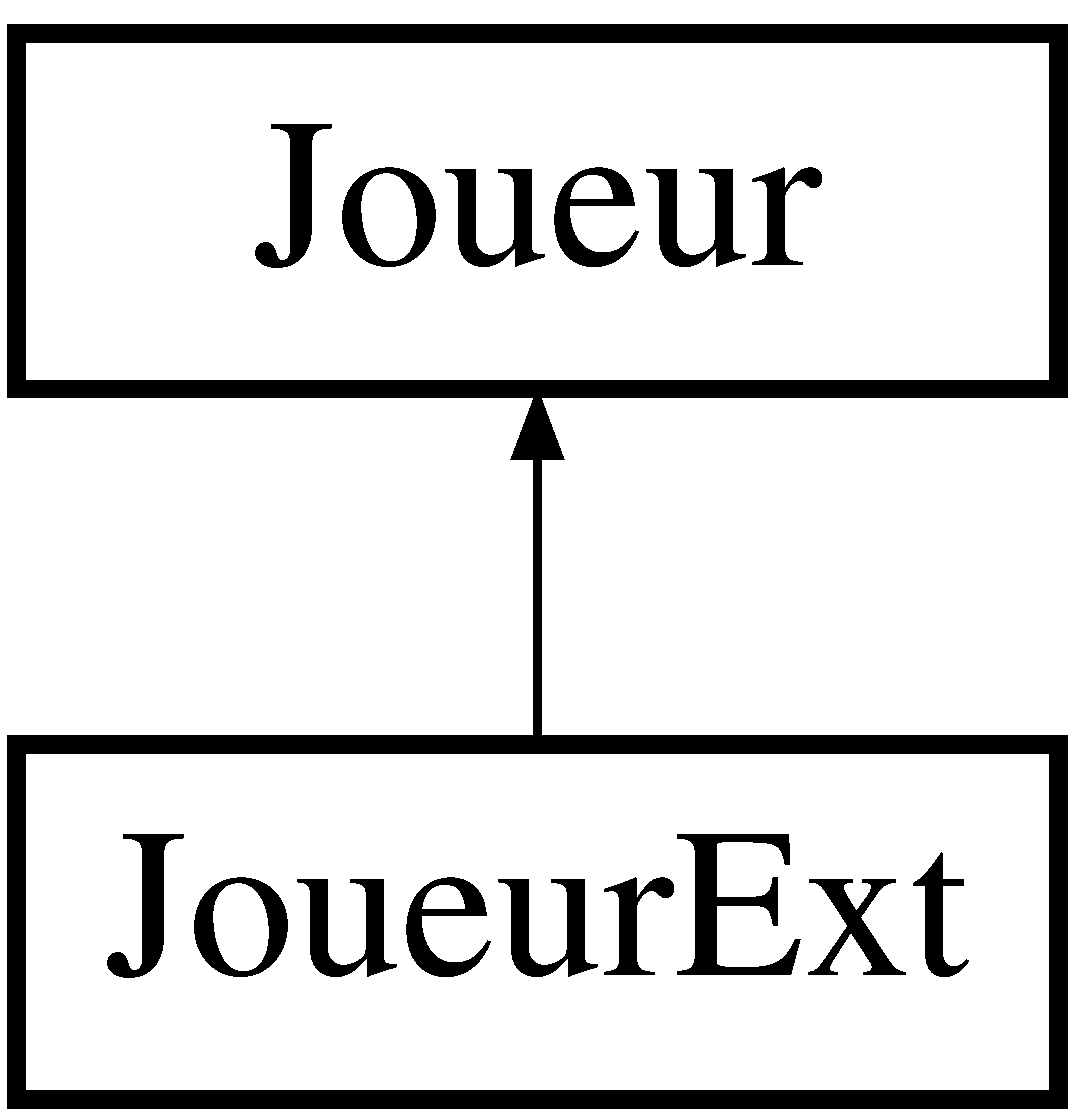
\includegraphics[height=2.000000cm]{classJoueur}
\end{center}
\end{figure}
\subsection*{Fonctions membres publiques}
\begin{DoxyCompactItemize}
\item 
\hypertarget{classJoueur_a87d494582f5a79f5b9e488b933342123}{\hyperlink{classJoueur_a87d494582f5a79f5b9e488b933342123}{Joueur} (float, float, float, bool)}\label{classJoueur_a87d494582f5a79f5b9e488b933342123}

\begin{DoxyCompactList}\small\item\em Créé un joueur (local) \end{DoxyCompactList}\item 
\hypertarget{classJoueur_a48131f41f401d5bc8ba619cc6501fefb}{void \hyperlink{classJoueur_a48131f41f401d5bc8ba619cc6501fefb}{avancer} (float, float, float)}\label{classJoueur_a48131f41f401d5bc8ba619cc6501fefb}

\begin{DoxyCompactList}\small\item\em Permet d'avancer le joueur. \end{DoxyCompactList}\item 
\hypertarget{classJoueur_a00e986852193988432d5bd7bd0f39280}{void \hyperlink{classJoueur_a00e986852193988432d5bd7bd0f39280}{reculer} (float, float, float)}\label{classJoueur_a00e986852193988432d5bd7bd0f39280}

\begin{DoxyCompactList}\small\item\em Permet de reculer le joueur. \end{DoxyCompactList}\item 
\hypertarget{classJoueur_a9879f99716a2e8c3379bb50da2f9003c}{void \hyperlink{classJoueur_a9879f99716a2e8c3379bb50da2f9003c}{gauche} (float, float, float)}\label{classJoueur_a9879f99716a2e8c3379bb50da2f9003c}

\begin{DoxyCompactList}\small\item\em Permet de déplacer vers la gauche le joueur. \end{DoxyCompactList}\item 
\hypertarget{classJoueur_a7cc3a3760137a4af263f8c280a32543e}{void \hyperlink{classJoueur_a7cc3a3760137a4af263f8c280a32543e}{droite} (float, float, float)}\label{classJoueur_a7cc3a3760137a4af263f8c280a32543e}

\begin{DoxyCompactList}\small\item\em Permet de déplacer vers la droite le joueur. \end{DoxyCompactList}\item 
\hypertarget{classJoueur_ab37feae3df59b6af024642660a216628}{void \hyperlink{classJoueur_ab37feae3df59b6af024642660a216628}{maj} (float, float)}\label{classJoueur_ab37feae3df59b6af024642660a216628}

\begin{DoxyCompactList}\small\item\em met à jour la position du regard (caméra) \end{DoxyCompactList}\item 
\hypertarget{classJoueur_a49cea54853cb00bfa6d202e85c28b423}{float {\bfseries get\-Posx} ()}\label{classJoueur_a49cea54853cb00bfa6d202e85c28b423}

\item 
\hypertarget{classJoueur_a0603bac92c9d01c2ffd41458cdfc0e12}{float {\bfseries get\-Posy} ()}\label{classJoueur_a0603bac92c9d01c2ffd41458cdfc0e12}

\item 
\hypertarget{classJoueur_a95ed54abb559304fb3cb0af4aa66ba9b}{float {\bfseries get\-Posz} ()}\label{classJoueur_a95ed54abb559304fb3cb0af4aa66ba9b}

\item 
\hypertarget{classJoueur_a09fa10f7ae974b01ce1b7cb368e4bb95}{float {\bfseries get\-Pos\-Camx} ()}\label{classJoueur_a09fa10f7ae974b01ce1b7cb368e4bb95}

\item 
\hypertarget{classJoueur_a8b87552f137fb3db5113ef179b38513c}{float {\bfseries get\-Pos\-Camy} ()}\label{classJoueur_a8b87552f137fb3db5113ef179b38513c}

\item 
\hypertarget{classJoueur_a794e13d55e087458595f01390d35525d}{float {\bfseries get\-Pos\-Camz} ()}\label{classJoueur_a794e13d55e087458595f01390d35525d}

\item 
\hypertarget{classJoueur_a5f07d780788f070ac9a03654e354baef}{void {\bfseries set\-Posz} (float)}\label{classJoueur_a5f07d780788f070ac9a03654e354baef}

\end{DoxyCompactItemize}
\subsection*{Attributs protégés}
\begin{DoxyCompactItemize}
\item 
\hypertarget{classJoueur_aa6f729cb2f752814353d67b934da0fcc}{float {\bfseries posx}}\label{classJoueur_aa6f729cb2f752814353d67b934da0fcc}

\item 
\hypertarget{classJoueur_a5c41b447033ee563da583db447934ec6}{float {\bfseries posy}}\label{classJoueur_a5c41b447033ee563da583db447934ec6}

\item 
\hypertarget{classJoueur_a54ce6f968bd1e8ae328b9af265c70e5f}{float {\bfseries posz}}\label{classJoueur_a54ce6f968bd1e8ae328b9af265c70e5f}

\item 
\hypertarget{classJoueur_aa7dcfa3ec6a3b1858f026c6dbab97d9d}{float {\bfseries camx}}\label{classJoueur_aa7dcfa3ec6a3b1858f026c6dbab97d9d}

\item 
\hypertarget{classJoueur_af1853f3becb17602b775f27d5abaf044}{float {\bfseries camy}}\label{classJoueur_af1853f3becb17602b775f27d5abaf044}

\item 
\hypertarget{classJoueur_a516bd192f0d2407f037834f781d95d76}{float {\bfseries camz}}\label{classJoueur_a516bd192f0d2407f037834f781d95d76}

\item 
\hypertarget{classJoueur_ac8d5dfba7ccd45c19df99b3aae83c897}{bool {\bfseries godmod}}\label{classJoueur_ac8d5dfba7ccd45c19df99b3aae83c897}

\end{DoxyCompactItemize}


La documentation de cette classe a été générée à partir des fichiers suivants \-:\begin{DoxyCompactItemize}
\item 
/home/xyrodileas/\-Bureau/\-Projet\-\_\-\-Graphique/trunk/code\-\_\-source/src/\-Joueur/Joueur.\-h\item 
/home/xyrodileas/\-Bureau/\-Projet\-\_\-\-Graphique/trunk/code\-\_\-source/src/\-Joueur/Joueur.\-cpp\end{DoxyCompactItemize}

\hypertarget{classJoueurExt}{\section{Référence de la classe Joueur\-Ext}
\label{classJoueurExt}\index{Joueur\-Ext@{Joueur\-Ext}}
}
Graphe d'héritage de Joueur\-Ext\-:\begin{figure}[H]
\begin{center}
\leavevmode
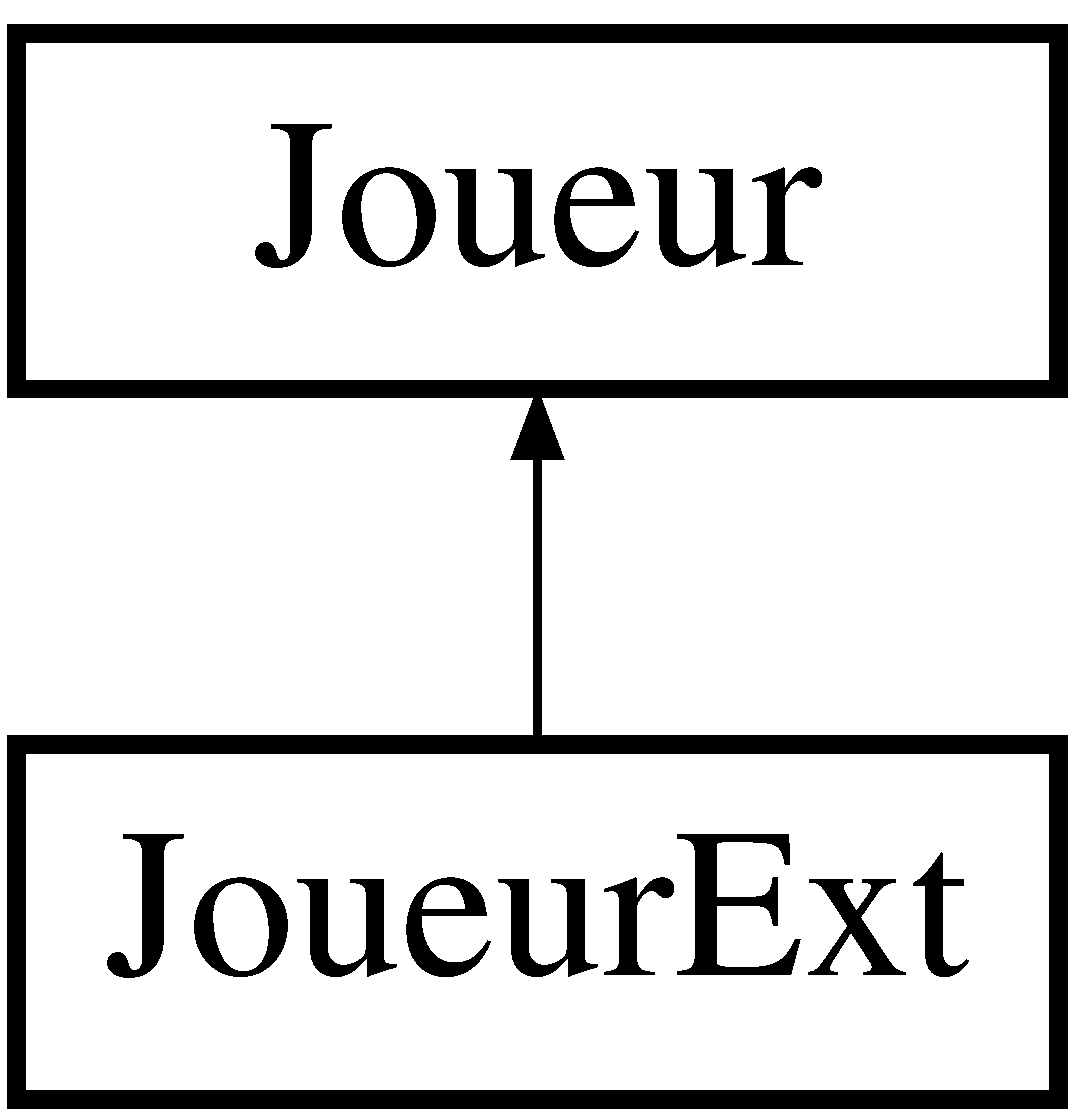
\includegraphics[height=2.000000cm]{classJoueurExt}
\end{center}
\end{figure}
\subsection*{Fonctions membres publiques}
\begin{DoxyCompactItemize}
\item 
\hypertarget{classJoueurExt_a6aaf4d501909088035eab7c30976c56b}{{\bfseries Joueur\-Ext} (float, float, float, bool, char $\ast$$\ast$)}\label{classJoueurExt_a6aaf4d501909088035eab7c30976c56b}

\item 
\hypertarget{classJoueurExt_a6b42376ef9dad3b028fe60452eac9ae2}{float {\bfseries get\-Pos\-Regardx} ()}\label{classJoueurExt_a6b42376ef9dad3b028fe60452eac9ae2}

\item 
\hypertarget{classJoueurExt_a6b7ca10441fe1bd4ae6b5bbfdf569a24}{float {\bfseries get\-Pos\-Regardy} ()}\label{classJoueurExt_a6b7ca10441fe1bd4ae6b5bbfdf569a24}

\item 
\hypertarget{classJoueurExt_adc14d839661cc6cdedb3cdd5b408adb4}{float {\bfseries get\-Pos\-Regardz} ()}\label{classJoueurExt_adc14d839661cc6cdedb3cdd5b408adb4}

\item 
\hypertarget{classJoueurExt_ac199a3646acea6924888e3bff11875f1}{void {\bfseries set\-Pos\-Regard} (int, int, int)}\label{classJoueurExt_ac199a3646acea6924888e3bff11875f1}

\item 
\hypertarget{classJoueurExt_a0d96b0535c075451f879839944c831fa}{void {\bfseries set\-Pos\-Joueur} (int, int, int)}\label{classJoueurExt_a0d96b0535c075451f879839944c831fa}

\item 
\hypertarget{classJoueurExt_ace7030a94124f4053c25644a095ae536}{char $\ast$$\ast$ {\bfseries get\-Pseudo} ()}\label{classJoueurExt_ace7030a94124f4053c25644a095ae536}

\item 
\hypertarget{classJoueurExt_ace82d1687f7c862e03f99f1d52bb8b74}{void {\bfseries set\-Pseudo} (char $\ast$$\ast$)}\label{classJoueurExt_ace82d1687f7c862e03f99f1d52bb8b74}

\item 
\hypertarget{classJoueurExt_a3f4da3fc59fc11dfea1ae62d7fc7dd7f}{void {\bfseries Draw\-Joueur} ()}\label{classJoueurExt_a3f4da3fc59fc11dfea1ae62d7fc7dd7f}

\end{DoxyCompactItemize}
\subsection*{Attributs protégés}
\begin{DoxyCompactItemize}
\item 
\hypertarget{classJoueurExt_a7a17662c22b6575d3497beca9510bbaf}{char $\ast$$\ast$ {\bfseries pseudo}}\label{classJoueurExt_a7a17662c22b6575d3497beca9510bbaf}

\end{DoxyCompactItemize}


La documentation de cette classe a été générée à partir des fichiers suivants \-:\begin{DoxyCompactItemize}
\item 
/home/xyrodileas/\-Bureau/\-Projet\-\_\-\-Graphique/trunk/code\-\_\-source/src/\-Joueur/Joueur\-Ext.\-h\item 
/home/xyrodileas/\-Bureau/\-Projet\-\_\-\-Graphique/trunk/code\-\_\-source/src/\-Joueur/Joueur\-Ext.\-cpp\end{DoxyCompactItemize}

\hypertarget{classMembre}{\section{Référence de la classe Membre}
\label{classMembre}\index{Membre@{Membre}}
}
\subsection*{Fonctions membres publiques}
\begin{DoxyCompactItemize}
\item 
\hypertarget{classMembre_aa6aef46a2d6c52f78a92d907f5456c3c}{{\bfseries Membre} (int, int, int, int, int, int, int, int, int)}\label{classMembre_aa6aef46a2d6c52f78a92d907f5456c3c}

\item 
\hypertarget{classMembre_aac479ed1be4d8439d91361f2cf406274}{void {\bfseries construire\-\_\-membre} ()}\label{classMembre_aac479ed1be4d8439d91361f2cf406274}

\item 
\hypertarget{classMembre_a8f12ab3b7c4f94e759bb8b1e5a86ebde}{int {\bfseries get\-X} ()}\label{classMembre_a8f12ab3b7c4f94e759bb8b1e5a86ebde}

\item 
\hypertarget{classMembre_a90ea50771ad39377e1f0cd398cdc804c}{int {\bfseries get\-Y} ()}\label{classMembre_a90ea50771ad39377e1f0cd398cdc804c}

\item 
\hypertarget{classMembre_aa343eb2632eaa24fe476eb86376fb0b8}{int {\bfseries get\-Z} ()}\label{classMembre_aa343eb2632eaa24fe476eb86376fb0b8}

\end{DoxyCompactItemize}
\subsection*{Fonctions membres protégées}
\begin{DoxyCompactItemize}
\item 
\hypertarget{classMembre_aa087f4c8a5338863f038e17dbcdcdd3e}{void {\bfseries initialiser\-\_\-membre} ()}\label{classMembre_aa087f4c8a5338863f038e17dbcdcdd3e}

\end{DoxyCompactItemize}
\subsection*{Attributs protégés}
\begin{DoxyCompactItemize}
\item 
\hypertarget{classMembre_a04ac42e599f243f78272a3c8e49b9e03}{int {\bfseries x}}\label{classMembre_a04ac42e599f243f78272a3c8e49b9e03}

\item 
\hypertarget{classMembre_a6f973cc67e074d031ae2531716f9361c}{int {\bfseries y}}\label{classMembre_a6f973cc67e074d031ae2531716f9361c}

\item 
\hypertarget{classMembre_adf58c4769c5d0c6c9b4e9b7581d4699c}{int {\bfseries z}}\label{classMembre_adf58c4769c5d0c6c9b4e9b7581d4699c}

\item 
\hypertarget{classMembre_a12bc2f7c0e74d2db178eaa2d04b9272a}{int {\bfseries largeur}}\label{classMembre_a12bc2f7c0e74d2db178eaa2d04b9272a}

\item 
\hypertarget{classMembre_aafc42963d0eadaa4d14524fc4463467b}{int {\bfseries longueur}}\label{classMembre_aafc42963d0eadaa4d14524fc4463467b}

\item 
\hypertarget{classMembre_ac99d101f9c39188cf0ca09a5e927bdbc}{int {\bfseries hauteur}}\label{classMembre_ac99d101f9c39188cf0ca09a5e927bdbc}

\item 
\hypertarget{classMembre_a5bfecfe7ee9f81e5757cac9e53447d8f}{int {\bfseries rouge}}\label{classMembre_a5bfecfe7ee9f81e5757cac9e53447d8f}

\item 
\hypertarget{classMembre_a26e2eeeeec8d1650b7acec77d8810c03}{int {\bfseries vert}}\label{classMembre_a26e2eeeeec8d1650b7acec77d8810c03}

\item 
\hypertarget{classMembre_a197a326ca4da8ef107273b469ce6d998}{int {\bfseries bleu}}\label{classMembre_a197a326ca4da8ef107273b469ce6d998}

\item 
\hypertarget{classMembre_a2170d897e6d3f78145b6ab21c768f5b4}{\hyperlink{classFace}{Face} $\ast$ {\bfseries avant}}\label{classMembre_a2170d897e6d3f78145b6ab21c768f5b4}

\item 
\hypertarget{classMembre_af4a7bb9ec540828b81be7d884f6d5b0d}{\hyperlink{classFace}{Face} $\ast$ {\bfseries arriere}}\label{classMembre_af4a7bb9ec540828b81be7d884f6d5b0d}

\item 
\hypertarget{classMembre_a822affb2c9c922cdaadaf73b63d54de4}{\hyperlink{classFace}{Face} $\ast$ {\bfseries dessous}}\label{classMembre_a822affb2c9c922cdaadaf73b63d54de4}

\item 
\hypertarget{classMembre_a85dae0ff7b515965fa2dc7f3a99b7efb}{\hyperlink{classFace}{Face} $\ast$ {\bfseries dessus}}\label{classMembre_a85dae0ff7b515965fa2dc7f3a99b7efb}

\item 
\hypertarget{classMembre_ad39f9dc6447e687bb1ac3f5c6cf50f1d}{\hyperlink{classFace}{Face} $\ast$ {\bfseries gauche}}\label{classMembre_ad39f9dc6447e687bb1ac3f5c6cf50f1d}

\item 
\hypertarget{classMembre_a4e4b1a707119e9edc9c24827447bfc99}{\hyperlink{classFace}{Face} $\ast$ {\bfseries droite}}\label{classMembre_a4e4b1a707119e9edc9c24827447bfc99}

\end{DoxyCompactItemize}


La documentation de cette classe a été générée à partir des fichiers suivants \-:\begin{DoxyCompactItemize}
\item 
/home/xyrodileas/\-Bureau/\-Projet\-\_\-\-Graphique/trunk/code\-\_\-source/src/personnage/Membre.\-h\item 
/home/xyrodileas/\-Bureau/\-Projet\-\_\-\-Graphique/trunk/code\-\_\-source/src/personnage/Membre.\-cpp\end{DoxyCompactItemize}

\hypertarget{classNetworkingException}{\section{Référence de la classe Networking\-Exception}
\label{classNetworkingException}\index{Networking\-Exception@{Networking\-Exception}}
}


{\ttfamily \#include $<$Networking\-Exception.\-hpp$>$}

\subsection*{Fonctions membres publiques}
\begin{DoxyCompactItemize}
\item 
\hypertarget{classNetworkingException_a81df7876959eab09308e492dc80c246f}{{\bfseries Networking\-Exception} (unsigned int ex)}\label{classNetworkingException_a81df7876959eab09308e492dc80c246f}

\item 
\hypertarget{classNetworkingException_aa1ce39b8840024c58af2d30cebcb27cc}{{\bfseries Networking\-Exception} (unsigned int ex, std\-::string c)}\label{classNetworkingException_aa1ce39b8840024c58af2d30cebcb27cc}

\item 
\hypertarget{classNetworkingException_aaff78085c8d2c91b3935f8280709bac5}{{\bfseries Networking\-Exception} (unsigned int ex, std\-::string m, std\-::string c)}\label{classNetworkingException_aaff78085c8d2c91b3935f8280709bac5}

\item 
\hypertarget{classNetworkingException_a8d04287652099fa29795b95e674d41dd}{{\bfseries Networking\-Exception} (std\-::string m)}\label{classNetworkingException_a8d04287652099fa29795b95e674d41dd}

\item 
\hypertarget{classNetworkingException_a29d2a57ce7bfd4ab9b8125bd5151f592}{std\-::string {\bfseries get\-Message} ()}\label{classNetworkingException_a29d2a57ce7bfd4ab9b8125bd5151f592}

\item 
\hypertarget{classNetworkingException_a8b4de44e6e8a2456917543bec8b95c68}{std\-::string {\bfseries get\-\_\-cause} ()}\label{classNetworkingException_a8b4de44e6e8a2456917543bec8b95c68}

\item 
void \hyperlink{classNetworkingException_ac5b663a69dff4cce3c5be45a6e245eb4}{display\-Sortie\-Standard2} ()
\end{DoxyCompactItemize}
\subsection*{Fonctions membres publiques statiques}
\begin{DoxyCompactItemize}
\item 
static void \hyperlink{classNetworkingException_acd20cabe5e9130c7798ce045eda1b931}{init\-\_\-err} ()
\end{DoxyCompactItemize}


\subsection{Description détaillée}
Cette classe permet de gérer des exeptions. Specialise dans les erreurs de reseau, elle peut aussi etre utilise pour n'importe quel type d'erreur. 

\subsection{Documentation des fonctions membres}
\hypertarget{classNetworkingException_ac5b663a69dff4cce3c5be45a6e245eb4}{\index{Networking\-Exception@{Networking\-Exception}!display\-Sortie\-Standard2@{display\-Sortie\-Standard2}}
\index{display\-Sortie\-Standard2@{display\-Sortie\-Standard2}!NetworkingException@{Networking\-Exception}}
\subsubsection[{display\-Sortie\-Standard2}]{\setlength{\rightskip}{0pt plus 5cm}void Networking\-Exception\-::display\-Sortie\-Standard2 (
\begin{DoxyParamCaption}
{}
\end{DoxyParamCaption}
)\hspace{0.3cm}{\ttfamily [inline]}}}\label{classNetworkingException_ac5b663a69dff4cce3c5be45a6e245eb4}
Affichage sur la sortie standard avec cout \hypertarget{classNetworkingException_acd20cabe5e9130c7798ce045eda1b931}{\index{Networking\-Exception@{Networking\-Exception}!init\-\_\-err@{init\-\_\-err}}
\index{init\-\_\-err@{init\-\_\-err}!NetworkingException@{Networking\-Exception}}
\subsubsection[{init\-\_\-err}]{\setlength{\rightskip}{0pt plus 5cm}void Networking\-Exception\-::init\-\_\-err (
\begin{DoxyParamCaption}
{}
\end{DoxyParamCaption}
)\hspace{0.3cm}{\ttfamily [inline]}, {\ttfamily [static]}}}\label{classNetworkingException_acd20cabe5e9130c7798ce045eda1b931}
Si {\itshape Je\-\_\-serai\-\_\-inclus} est definie alors les variables seront importe au moment du linkage Initialise les erreurs en fonction d'un identifiant Identifiants entre 0 et 99 (inclus) ==$>$ le serveur parle Identifiants superieurs a 99 ==$>$ le client parle 

La documentation de cette classe a été générée à partir du fichier suivant \-:\begin{DoxyCompactItemize}
\item 
/home/xyrodileas/\-Bureau/\-Projet\-\_\-\-Graphique/trunk/code\-\_\-source/src/reseau/Networking\-Exception.\-hpp\end{DoxyCompactItemize}

\hypertarget{classPersonnage}{\section{Référence de la classe Personnage}
\label{classPersonnage}\index{Personnage@{Personnage}}
}
\subsection*{Fonctions membres publiques}
\begin{DoxyCompactItemize}
\item 
\hypertarget{classPersonnage_afba39eec21ceedcf8e5c5db996438b2e}{{\bfseries Personnage} (int, int, int, int, int, int)}\label{classPersonnage_afba39eec21ceedcf8e5c5db996438b2e}

\item 
\hypertarget{classPersonnage_af2b2a8412f4f9b9291b289fbccd00c14}{void {\bfseries construire\-\_\-personnage} ()}\label{classPersonnage_af2b2a8412f4f9b9291b289fbccd00c14}

\end{DoxyCompactItemize}
\subsection*{Fonctions membres protégées}
\begin{DoxyCompactItemize}
\item 
\hypertarget{classPersonnage_a1b33c2388a3bd03f6137f03e91a61bab}{void {\bfseries construire\-\_\-corps} ()}\label{classPersonnage_a1b33c2388a3bd03f6137f03e91a61bab}

\item 
\hypertarget{classPersonnage_a5bc2b2cea92e8f5316bc7268bc6ae391}{void {\bfseries initialiser\-\_\-personnage} ()}\label{classPersonnage_a5bc2b2cea92e8f5316bc7268bc6ae391}

\end{DoxyCompactItemize}
\subsection*{Attributs protégés}
\begin{DoxyCompactItemize}
\item 
\hypertarget{classPersonnage_aed98af55dd1a3b21c5a446713061b67e}{int {\bfseries x}}\label{classPersonnage_aed98af55dd1a3b21c5a446713061b67e}

\item 
\hypertarget{classPersonnage_a4fdc0728efe8d50059d81a7672c86555}{int {\bfseries y}}\label{classPersonnage_a4fdc0728efe8d50059d81a7672c86555}

\item 
\hypertarget{classPersonnage_ad3d37fb897ae674345b01d7497ec47ee}{int {\bfseries z}}\label{classPersonnage_ad3d37fb897ae674345b01d7497ec47ee}

\item 
\hypertarget{classPersonnage_a504d98f78c1d5022ac164caf7aacba08}{int {\bfseries largeur}}\label{classPersonnage_a504d98f78c1d5022ac164caf7aacba08}

\item 
\hypertarget{classPersonnage_ad8e61921f34f7680f17f55921a193b3a}{int {\bfseries longueur}}\label{classPersonnage_ad8e61921f34f7680f17f55921a193b3a}

\item 
\hypertarget{classPersonnage_a7bccfce1f1af9a06de5772ac8d348410}{int {\bfseries hauteur}}\label{classPersonnage_a7bccfce1f1af9a06de5772ac8d348410}

\item 
\hypertarget{classPersonnage_a7d0c0123fbf209ab95734eb411983c05}{\hyperlink{classMembre}{Membre} $\ast$ {\bfseries bras\-Droit}}\label{classPersonnage_a7d0c0123fbf209ab95734eb411983c05}

\item 
\hypertarget{classPersonnage_a0451c170fb5aa61bfff6557ac841dd50}{\hyperlink{classMembre}{Membre} $\ast$ {\bfseries bras\-Gauche}}\label{classPersonnage_a0451c170fb5aa61bfff6557ac841dd50}

\item 
\hypertarget{classPersonnage_ab0510f00b730cc50e355774d74015c84}{\hyperlink{classMembre}{Membre} $\ast$ {\bfseries tete}}\label{classPersonnage_ab0510f00b730cc50e355774d74015c84}

\item 
\hypertarget{classPersonnage_a7b9c48d3b0ddab27701c81c172ab32ed}{\hyperlink{classMembre}{Membre} $\ast$ {\bfseries corps}}\label{classPersonnage_a7b9c48d3b0ddab27701c81c172ab32ed}

\item 
\hypertarget{classPersonnage_a1040b2d31632282687518094f7fbf1e8}{\hyperlink{classMembre}{Membre} $\ast$ {\bfseries jambe\-Droite}}\label{classPersonnage_a1040b2d31632282687518094f7fbf1e8}

\item 
\hypertarget{classPersonnage_a3c68d1eed6ae3d91aac3d5594ae86f7f}{\hyperlink{classMembre}{Membre} $\ast$ {\bfseries jambe\-Gauche}}\label{classPersonnage_a3c68d1eed6ae3d91aac3d5594ae86f7f}

\end{DoxyCompactItemize}


La documentation de cette classe a été générée à partir des fichiers suivants \-:\begin{DoxyCompactItemize}
\item 
/home/xyrodileas/\-Bureau/\-Projet\-\_\-\-Graphique/trunk/code\-\_\-source/src/personnage/Personnage.\-h\item 
/home/xyrodileas/\-Bureau/\-Projet\-\_\-\-Graphique/trunk/code\-\_\-source/src/personnage/Personnage.\-cpp\end{DoxyCompactItemize}

\hypertarget{classPlateau}{\section{Référence de la classe Plateau}
\label{classPlateau}\index{Plateau@{Plateau}}
}
\subsection*{Fonctions membres publiques}
\begin{DoxyCompactItemize}
\item 
\hypertarget{classPlateau_ab0ce9c3f8d8644c622890366ceb478c8}{{\bfseries Plateau} (int, int, int, float)}\label{classPlateau_ab0ce9c3f8d8644c622890366ceb478c8}

\item 
\hypertarget{classPlateau_a33ebd454a5a1471401c715b7069efb69}{void \hyperlink{classPlateau_a33ebd454a5a1471401c715b7069efb69}{afficher\-\_\-plateau} ()}\label{classPlateau_a33ebd454a5a1471401c715b7069efb69}

\begin{DoxyCompactList}\small\item\em permet d'afficher le plateau avec opengl \end{DoxyCompactList}\item 
\hypertarget{classPlateau_a2448e265658f9ba1395b1a5961d0e70c}{void \hyperlink{classPlateau_a2448e265658f9ba1395b1a5961d0e70c}{supprimer\-\_\-cube} (int, int, int)}\label{classPlateau_a2448e265658f9ba1395b1a5961d0e70c}

\begin{DoxyCompactList}\small\item\em Permet de supprimer un cube de la map. \end{DoxyCompactList}\item 
\hypertarget{classPlateau_ad31477b73aec12d467075db6a1f24530}{void \hyperlink{classPlateau_ad31477b73aec12d467075db6a1f24530}{ajouter\-\_\-cube} (int, int, int)}\label{classPlateau_ad31477b73aec12d467075db6a1f24530}

\begin{DoxyCompactList}\small\item\em Permet d'ajouter un cube sur la map. \end{DoxyCompactList}\item 
\hypertarget{classPlateau_a1ee031a882c90fa2a82c115c7eedd844}{void \hyperlink{classPlateau_a1ee031a882c90fa2a82c115c7eedd844}{verifier\-\_\-integrite\-\_\-cubes} ()}\label{classPlateau_a1ee031a882c90fa2a82c115c7eedd844}

\begin{DoxyCompactList}\small\item\em Vérifie l'intégrité du plateau (méthode de test) \end{DoxyCompactList}\item 
\hypertarget{classPlateau_a8ae0bfe889dd6612ef0054f2e04ed5be}{bool \hyperlink{classPlateau_a8ae0bfe889dd6612ef0054f2e04ed5be}{is\-Cube} (int, int, int)}\label{classPlateau_a8ae0bfe889dd6612ef0054f2e04ed5be}

\begin{DoxyCompactList}\small\item\em Permet de vérifier s'il y a un cube (Utilisé pour la détection des colisions) \end{DoxyCompactList}\end{DoxyCompactItemize}


La documentation de cette classe a été générée à partir des fichiers suivants \-:\begin{DoxyCompactItemize}
\item 
/home/xyrodileas/\-Bureau/\-Projet\-\_\-\-Graphique/trunk/code\-\_\-source/src/plateau/Plateau.\-h\item 
/home/xyrodileas/\-Bureau/\-Projet\-\_\-\-Graphique/trunk/code\-\_\-source/src/plateau/Plateau.\-cpp\end{DoxyCompactItemize}

\hypertarget{classPoint}{\section{Référence de la classe Point}
\label{classPoint}\index{Point@{Point}}
}
\subsection*{Fonctions membres publiques}
\begin{DoxyCompactItemize}
\item 
\hypertarget{classPoint_a326edb72707d198c949cde90dcd3557a}{{\bfseries Point} (float, float, float)}\label{classPoint_a326edb72707d198c949cde90dcd3557a}

\item 
\hypertarget{classPoint_aecfc6968998d806384e24cd93072b024}{\hyperlink{classPoint}{Point} \& {\bfseries operator=} (const \hyperlink{classPoint}{Point} \&)}\label{classPoint_aecfc6968998d806384e24cd93072b024}

\item 
\hypertarget{classPoint_acc27466778cc87a662bba40268c4c0c8}{float {\bfseries get\-X} ()}\label{classPoint_acc27466778cc87a662bba40268c4c0c8}

\item 
\hypertarget{classPoint_a3cccbca94719ddde353cce86ce0e2f64}{float {\bfseries get\-Y} ()}\label{classPoint_a3cccbca94719ddde353cce86ce0e2f64}

\item 
\hypertarget{classPoint_adfd464bbfabdcecdcc14eb83cf6d2830}{float {\bfseries get\-Z} ()}\label{classPoint_adfd464bbfabdcecdcc14eb83cf6d2830}

\item 
\hypertarget{classPoint_a61253b28283b54a9cf379132bdff3006}{void {\bfseries set\-X} (float)}\label{classPoint_a61253b28283b54a9cf379132bdff3006}

\item 
\hypertarget{classPoint_a0a9d3529888cd2fd7c0adb8e46702110}{void {\bfseries set\-Y} (float)}\label{classPoint_a0a9d3529888cd2fd7c0adb8e46702110}

\item 
\hypertarget{classPoint_acaf34d6d8ca4ef7e50c6d75ff54f9516}{void {\bfseries set\-Z} (float)}\label{classPoint_acaf34d6d8ca4ef7e50c6d75ff54f9516}

\end{DoxyCompactItemize}
\subsection*{Attributs protégés}
\begin{DoxyCompactItemize}
\item 
\hypertarget{classPoint_a05dfe2dfbde813ad234b514f30e662f1}{float {\bfseries x}}\label{classPoint_a05dfe2dfbde813ad234b514f30e662f1}

\item 
\hypertarget{classPoint_a6101960c8d2d4e8ea1d32c9234bbeb8d}{float {\bfseries y}}\label{classPoint_a6101960c8d2d4e8ea1d32c9234bbeb8d}

\item 
\hypertarget{classPoint_a9a666531e0e99adff132be93d2407d0c}{float {\bfseries z}}\label{classPoint_a9a666531e0e99adff132be93d2407d0c}

\end{DoxyCompactItemize}


La documentation de cette classe a été générée à partir des fichiers suivants \-:\begin{DoxyCompactItemize}
\item 
/home/xyrodileas/\-Bureau/\-Projet\-\_\-\-Graphique/trunk/code\-\_\-source/src/cube/Point.\-h\item 
/home/xyrodileas/\-Bureau/\-Projet\-\_\-\-Graphique/trunk/code\-\_\-source/src/cube/Point.\-cpp\end{DoxyCompactItemize}

\hypertarget{classServeur}{\section{Référence de la classe Serveur}
\label{classServeur}\index{Serveur@{Serveur}}
}


{\ttfamily \#include $<$reseau.\-hpp$>$}

\subsection*{Classes}
\begin{DoxyCompactItemize}
\item 
struct {\bfseries Ecoute}
\end{DoxyCompactItemize}
\subsection*{Fonctions membres publiques}
\begin{DoxyCompactItemize}
\item 
\hyperlink{classServeur_a8a7a1df15a07e095436dedd0d40a0196}{Serveur} ()
\item 
void \hyperlink{classServeur_a7421ed36dd73bad688ef617b684688a7}{kick} (std\-::string)
\item 
void \hyperlink{classServeur_a88c66169c035dd9fb1d7a220e32b99f6}{clients} ()
\item 
\hypertarget{classServeur_af7bcbec1b825911c32f64eb9b2d23deb}{void {\bfseries csocks} ()}\label{classServeur_af7bcbec1b825911c32f64eb9b2d23deb}

\item 
\hypertarget{classServeur_ad2c277503a0abc4cb1a203340a055734}{void {\bfseries messagess} ()}\label{classServeur_ad2c277503a0abc4cb1a203340a055734}

\item 
\hyperlink{classServeur_a722aefd65c9efab0b3e0646bf3440ea1}{$\sim$\-Serveur} ()
\end{DoxyCompactItemize}
\subsection*{Amis}
\begin{DoxyCompactItemize}
\item 
void $\ast$ \hyperlink{classServeur_afb450ae26198b5e7e34d4e6d5939f9ee}{attente\-\_\-clients} (void $\ast$)
\item 
void $\ast$ \hyperlink{classServeur_ae17c0b8683120a4c6a61b5b38bed0225}{ecoute\-\_\-client} (void $\ast$)
\item 
void $\ast$ \hyperlink{classServeur_ac359cb70bf30e80424334f5c858f9d80}{ecoute\-\_\-clients} (void $\ast$)
\item 
void $\ast$ \hyperlink{classServeur_a3eb5f390c851d5db2e61b5bd5156b242}{envoi\-\_\-aux\-\_\-clients} (void $\ast$)
\end{DoxyCompactItemize}


\subsection{Description détaillée}
Include personnels La classe serveur gere beaucoup de choses toute seule. Se limiter aux fonction publique pour usage. 

\subsection{Documentation des constructeurs et destructeur}
\hypertarget{classServeur_a8a7a1df15a07e095436dedd0d40a0196}{\index{Serveur@{Serveur}!Serveur@{Serveur}}
\index{Serveur@{Serveur}!Serveur@{Serveur}}
\subsubsection[{Serveur}]{\setlength{\rightskip}{0pt plus 5cm}Serveur\-::\-Serveur (
\begin{DoxyParamCaption}
{}
\end{DoxyParamCaption}
)}}\label{classServeur_a8a7a1df15a07e095436dedd0d40a0196}
Le constructeur initialise les erreurs du Networking exception initialise la socket principale et lui donne un adressage creer un thread pour ecouter les demandes de connection des différents clients \hypertarget{classServeur_a722aefd65c9efab0b3e0646bf3440ea1}{\index{Serveur@{Serveur}!$\sim$\-Serveur@{$\sim$\-Serveur}}
\index{$\sim$\-Serveur@{$\sim$\-Serveur}!Serveur@{Serveur}}
\subsubsection[{$\sim$\-Serveur}]{\setlength{\rightskip}{0pt plus 5cm}Serveur\-::$\sim$\-Serveur (
\begin{DoxyParamCaption}
{}
\end{DoxyParamCaption}
)}}\label{classServeur_a722aefd65c9efab0b3e0646bf3440ea1}
Ferme les connexions et les threads lance avant la fermeture du serveur libere la memoire allouer pour les \char`\"{}new thread\-\_\-t\char`\"{} 

\subsection{Documentation des fonctions membres}
\hypertarget{classServeur_a88c66169c035dd9fb1d7a220e32b99f6}{\index{Serveur@{Serveur}!clients@{clients}}
\index{clients@{clients}!Serveur@{Serveur}}
\subsubsection[{clients}]{\setlength{\rightskip}{0pt plus 5cm}void Serveur\-::clients (
\begin{DoxyParamCaption}
{}
\end{DoxyParamCaption}
)\hspace{0.3cm}{\ttfamily [inline]}}}\label{classServeur_a88c66169c035dd9fb1d7a220e32b99f6}
Utilise seulement pour le debuggage \hypertarget{classServeur_a7421ed36dd73bad688ef617b684688a7}{\index{Serveur@{Serveur}!kick@{kick}}
\index{kick@{kick}!Serveur@{Serveur}}
\subsubsection[{kick}]{\setlength{\rightskip}{0pt plus 5cm}void Serveur\-::kick (
\begin{DoxyParamCaption}
\item[{std\-::string}]{nom}
\end{DoxyParamCaption}
)}}\label{classServeur_a7421ed36dd73bad688ef617b684688a7}
Comme sont nom l'indique, on sort le client du nom  

\subsection{Documentation des fonctions amies et associées}
\hypertarget{classServeur_afb450ae26198b5e7e34d4e6d5939f9ee}{\index{Serveur@{Serveur}!attente\-\_\-clients@{attente\-\_\-clients}}
\index{attente\-\_\-clients@{attente\-\_\-clients}!Serveur@{Serveur}}
\subsubsection[{attente\-\_\-clients}]{\setlength{\rightskip}{0pt plus 5cm}void$\ast$ attente\-\_\-clients (
\begin{DoxyParamCaption}
\item[{void $\ast$}]{arg}
\end{DoxyParamCaption}
)\hspace{0.3cm}{\ttfamily [friend]}}}\label{classServeur_afb450ae26198b5e7e34d4e6d5939f9ee}
Fonction ami de la classe serveur permettant la demade de connexion par les clients \hypertarget{classServeur_ae17c0b8683120a4c6a61b5b38bed0225}{\index{Serveur@{Serveur}!ecoute\-\_\-client@{ecoute\-\_\-client}}
\index{ecoute\-\_\-client@{ecoute\-\_\-client}!Serveur@{Serveur}}
\subsubsection[{ecoute\-\_\-client}]{\setlength{\rightskip}{0pt plus 5cm}void$\ast$ ecoute\-\_\-client (
\begin{DoxyParamCaption}
\item[{void $\ast$}]{arg}
\end{DoxyParamCaption}
)\hspace{0.3cm}{\ttfamily [friend]}}}\label{classServeur_ae17c0b8683120a4c6a61b5b38bed0225}
ecoute les messages de sont client attitre par  et insert les receptions dans messages C\-O\-D\-E T\-E\-S\-T E\-N\-L\-E\-V\-E\-R Q\-U\-A\-N\-D C\-O\-R\-R\-E\-C\-T\-E C\-O\-D\-E T\-E\-S\-T E\-N\-L\-E\-V\-E\-R Q\-U\-A\-N\-D C\-O\-R\-R\-E\-C\-T\-E C\-O\-D\-E T\-E\-S\-T E\-N\-L\-E\-V\-E\-R Q\-U\-A\-N\-D C\-O\-R\-R\-E\-C\-T\-E C\-O\-D\-E T\-E\-S\-T E\-N\-L\-E\-V\-E\-R Q\-U\-A\-N\-D C\-O\-R\-R\-E\-C\-T\-E C\-O\-D\-E T\-E\-S\-T E\-N\-L\-E\-V\-E\-R Q\-U\-A\-N\-D C\-O\-R\-R\-E\-C\-T\-E C\-O\-D\-E T\-E\-S\-T E\-N\-L\-E\-V\-E\-R Q\-U\-A\-N\-D C\-O\-R\-R\-E\-C\-T\-E C\-O\-D\-E T\-E\-S\-T E\-N\-L\-E\-V\-E\-R Q\-U\-A\-N\-D C\-O\-R\-R\-E\-C\-T\-E

C\-O\-D\-E T\-E\-S\-T E\-N\-L\-E\-V\-E\-R Q\-U\-A\-N\-D C\-O\-R\-R\-E\-C\-T\-E C\-O\-D\-E T\-E\-S\-T E\-N\-L\-E\-V\-E\-R Q\-U\-A\-N\-D C\-O\-R\-R\-E\-C\-T\-E C\-O\-D\-E T\-E\-S\-T E\-N\-L\-E\-V\-E\-R Q\-U\-A\-N\-D C\-O\-R\-R\-E\-C\-T\-E C\-O\-D\-E T\-E\-S\-T E\-N\-L\-E\-V\-E\-R Q\-U\-A\-N\-D C\-O\-R\-R\-E\-C\-T\-E C\-O\-D\-E T\-E\-S\-T E\-N\-L\-E\-V\-E\-R Q\-U\-A\-N\-D C\-O\-R\-R\-E\-C\-T\-E C\-O\-D\-E T\-E\-S\-T E\-N\-L\-E\-V\-E\-R Q\-U\-A\-N\-D C\-O\-R\-R\-E\-C\-T\-E\hypertarget{classServeur_ac359cb70bf30e80424334f5c858f9d80}{\index{Serveur@{Serveur}!ecoute\-\_\-clients@{ecoute\-\_\-clients}}
\index{ecoute\-\_\-clients@{ecoute\-\_\-clients}!Serveur@{Serveur}}
\subsubsection[{ecoute\-\_\-clients}]{\setlength{\rightskip}{0pt plus 5cm}void$\ast$ ecoute\-\_\-clients (
\begin{DoxyParamCaption}
\item[{void $\ast$}]{arg}
\end{DoxyParamCaption}
)\hspace{0.3cm}{\ttfamily [friend]}}}\label{classServeur_ac359cb70bf30e80424334f5c858f9d80}
Creer un thread d'ecoute par client \hypertarget{classServeur_a3eb5f390c851d5db2e61b5bd5156b242}{\index{Serveur@{Serveur}!envoi\-\_\-aux\-\_\-clients@{envoi\-\_\-aux\-\_\-clients}}
\index{envoi\-\_\-aux\-\_\-clients@{envoi\-\_\-aux\-\_\-clients}!Serveur@{Serveur}}
\subsubsection[{envoi\-\_\-aux\-\_\-clients}]{\setlength{\rightskip}{0pt plus 5cm}void$\ast$ envoi\-\_\-aux\-\_\-clients (
\begin{DoxyParamCaption}
\item[{void $\ast$}]{arg}
\end{DoxyParamCaption}
)\hspace{0.3cm}{\ttfamily [friend]}}}\label{classServeur_a3eb5f390c851d5db2e61b5bd5156b242}
Prend tout les messages stocké dans la base et les renvoi a tout les clients sauf l'emetteur 

La documentation de cette classe a été générée à partir des fichiers suivants \-:\begin{DoxyCompactItemize}
\item 
/home/xyrodileas/\-Bureau/\-Projet\-\_\-\-Graphique/trunk/code\-\_\-source/src/reseau/reseau.\-hpp\item 
/home/xyrodileas/\-Bureau/\-Projet\-\_\-\-Graphique/trunk/code\-\_\-source/src/reseau/server.\-cpp\end{DoxyCompactItemize}

\printindex
\end{document}
